\documentclass[xcolor=dvipsnames,table]{beamer}

\usepackage{latexsym}
\usepackage[utf8]{inputenc}
\usepackage[brazil]{babel}
\usepackage{amssymb}
\usepackage{amsmath}
\usepackage{stmaryrd}
\usepackage{fancybox}
\usepackage{datetime}
\usepackage[T1]{fontenc}
\usepackage{graphicx}
\usepackage{graphics}
\usepackage{url}
\usepackage{algorithmic}
\usepackage{algorithm}
\usepackage{acronym}
\usepackage{array}

\newtheorem{definicao}{Definio}
\newcommand{\tab}{\hspace*{2em}}

\mode<presentation>
{
  \definecolor{colortexto}{RGB}{0,0,0}
 
  \setbeamertemplate{background canvas}[vertical shading][ bottom=white!10,top=white!10]
  \setbeamercolor{normal text}{fg=colortexto} 

  \usetheme{Warsaw}
}

\title{Decidibilidade} 

\author{
  Esdras Lins Bispo Jr. \\ \url{bispojr@ufg.br}
  } 
 \institute{
  Teoria da Computação \\Bacharelado em Ciência da Computação}
\date{\textbf{13 de dezembro de 2017} }

\logo{
\includegraphics[width=1cm]{images/ufgJataiLogo.png}}

\begin{document}

	\begin{frame}
		\titlepage
	\end{frame}

	\AtBeginSection{
		\begin{frame}{Sumário}%[allowframebreaks]{Sumário}
    		\tableofcontents[currentsection]
    		%\tableofcontents[currentsection, hideothersubsections]
		\end{frame}
	}

	\begin{frame}{Plano de Aula}
		\tableofcontents
		%\tableofcontents[hideallsubsections]
	\end{frame}
	
	
%------------------------------------------
	\section{Revisão}
	\begin{frame}
		\begin{block}{Pergunta 1}
			Em relação à máquina de Turing, é {\bf incorreto} afirmar que...
		\end{block}
		\begin{enumerate}[(A)]
			\item Uma máquina de Turing pode tanto escrever sobre a fita quanto ler a partir dela.
			\item A cabeça de leitura–escrita pode mover-se tanto para a esquerda quanto para a direita.
			\item A fita é infinita.
			\item Os estados especiais para rejeitar e aceitar fazem efeito apenas após a leitura de toda a cadeia.
		\end{enumerate}
	\end{frame}

	\begin{frame}
		\begin{block}{Pergunta 2}
			O valor de retorno da função de transição $\delta$ de uma máquina de Turing é...
		\end{block}
		\begin{enumerate}[(A)]
			\item uma tripla contendo o estado de destino, o símbolo a ser escrito na fita e o movimento da cabeça.
			\item uma dupla contendo o símbolo a ser escrito na fita e o movimento da cabeça.
			\item uma tripla contendo o estado de origem, o símbolo a ser lido na fita e o movimento da cabeça.
			\item uma dupla contendo o símbolo a ser lido na fita e o movimento da cabeça.
		\end{enumerate}
	\end{frame}

	\begin{frame}
		\begin{block}{Pergunta 3}
			Sobre o alfabeto da fita $\Gamma$ e o alfabeto da linguagem $\Sigma$ é {\bf incorreto} afirmar que...
		\end{block}
		\begin{enumerate}[(A)]
			\item $\sqcup \in \Gamma$ 
			\item $\Gamma \subseteq \Sigma$
			\item $\Sigma \subseteq \Gamma$
			\item $\Sigma \subset \Gamma$
		\end{enumerate}
	\end{frame}

	\begin{frame}
		\begin{block}{Pergunta 4}
			Quantos estados, no mínimo, uma máquina de Turing pode ter?
		\end{block}
		\begin{enumerate}[(A)]
			\item um
			\item dois
			\item três
			\item nenhum
		\end{enumerate}
	\end{frame}

	\begin{frame}
		\begin{block}{Pergunta 5}
			Para se provar que a classe de linguagens decidíveis é fechada sob a operação de união, é necessário...
		\end{block}
		\begin{enumerate}[(A)]
			\item construir uma máquina de Turing que reconhece $A \cup B$, sendo $A$ e $B$ duas linguagens decidíveis quaisquer.
			\item construir a linguagem $A$ e a linguagem $B$, a partir de um decisor para $A \cup B$ qualquer.
			\item construir um decisor para $A \cup B$, sendo $A$ e $B$ duas linguagens decidíveis quaisquer.
			\item construir uma máquina de Turing que reconhece $A \cup B$, sendo $A$ e $B$ duas linguagens quaisquer.
		\end{enumerate}
	\end{frame}

	\begin{frame}
		\begin{block}{Pergunta 6}
			A classe de linguagens Turing-reconhecíveis {\bf não} é fechada sob a operação de complemento. Isto deve-se ao fato de...
		\end{block}
		\begin{enumerate}[(A)]
			\item uma máquina de Turing qualquer admitir a possibilidade de entrar em {\it loop} infinito.
			\item não termos conhecimento prévio sobre qual será a cadeia de entrada que será fornecida para a máquina.
			\item qualquer máquina de Turing ter uma fita infinita, não permitindo saber se a cadeia será aceita ou não pela máquina.
			\item termos que utilizar uma máquina de Turing de uma única fita (ao invés de uma multifita).
		\end{enumerate}
	\end{frame}

	\begin{frame}
		\begin{block}{Pergunta 7}
			O russo Yuri Matijasevic mostrou que era impossível conceber um algoritmo que testasse se um polinômio qualquer tem ou não raiz inteira. Em outros termos, ele provou que...
		\end{block}
		\begin{enumerate}[(A)]
			\item a linguagem associada a este problema não é Turing-reconhecível. 
			\item não existe uma máquina de Turing que reconheça a linguagem associada a este problema.
			\item não existe uma linguagem associada a este problema.
			\item não existe uma máquina de Turing que decida a linguagem associada a este problema.
		\end{enumerate}
	\end{frame}

	\begin{frame}
		\begin{block}{Pergunta 8}
			
			\begin{columns}
				\begin{column}{0.05\textwidth}\end{column}
				\begin{column}{0.45\textwidth}
					A maioria das estruturas de dados podem ser representadas por uma cadeia. Qual das alternativas {\bf não} é uma representação válida do grafo apresentado na figura ao lado?
				\end{column}
				\begin{column}{0.5\textwidth}  %%<--- here
					\begin{center}
						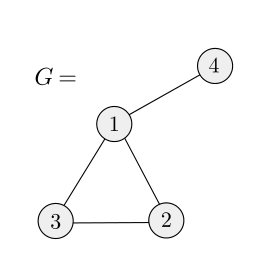
\includegraphics[width=.6\textwidth]{images/grafo}
					\end{center}
				\end{column}
			\end{columns}
			\begin{center}
				
			\end{center}
		\end{block}
		\begin{enumerate}[(A)]
			\item (1,2,3,4)((1,2),(2,3),(3,1),(1,4)) 
			\item (1\#2, 2\#3, 3\#1, 1\#4)
			\item 12, 23, 31, 14 / 1-3-4
			\item 12 - 23 - 31 - 14
		\end{enumerate}
	\end{frame}

	\section{Instrução pelos Colegas}
	\begin{frame}
		\begin{block}{Pergunta 1}
			O problema da aceitação procura compreender se...
		\end{block}
		\begin{enumerate}[(A)]
			\item uma cadeia descreve um modelo computacional.
			\item um modelo computacional reconhece expressões regulares.
			\item um modelo computacional aceita uma dada cadeia.
			\item uma cadeia é descrita por uma sequência de caracteres.
		\end{enumerate}
	\end{frame}

	\begin{frame}
		\begin{block}{Pergunta 2}
			Na linguagem $A_{AFD} = \{\langle B, \omega \rangle$ | $B$ é um AFD que aceita a cadeia de entrada $\omega \}$, qual é a afirmação {\bf incorreta} sobre ela?
		\end{block}
		\begin{enumerate}[(A)]
			\item A linguagem $A_{AFD}$ é um subconjunto de $L(B)$.
			\item $B$ é a codificação de um AFD.
			\item $A_{AFD}$ é a linguagem de todas as cadeias que contém a codificação de um AFD junto com uma cadeia que este AFD aceita.
			\item $\langle B, \omega \rangle$ é uma cadeia.
			
		\end{enumerate}
	\end{frame}

	\begin{frame}
		\begin{block}{Pergunta 3}
			\begin{columns}
				\begin{column}{0.05\textwidth}\end{column}
				\begin{column}{0.45\textwidth}
					Qual das alternativas está correta, em relação ao AFD $M$ ao lado?
				\end{column}
				\begin{column}{0.5\textwidth}  %%<--- here
					\begin{center}
						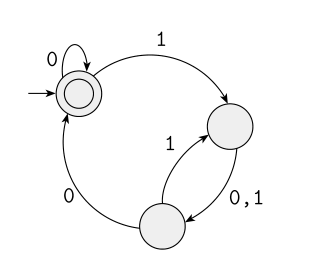
\includegraphics[width=.7\textwidth]{images/afd}
					\end{center}
				\end{column}
			\end{columns}
			\begin{center}
				
			\end{center}
		\end{block}
		\begin{enumerate}[(A)]
			\item $A_{AFD} \in \langle M, 0100 \rangle$
			\item $\langle M, 0100 \rangle \in A_{AFD}$ 
			\item $\langle 0100, M \rangle \in A_{AFD}$
			\item $A_{AFD} \in \langle 0100, M \rangle$
		\end{enumerate}
	\end{frame}

	\begin{frame}
		\titlepage
	\end{frame}
	
\end{document}